\subsection{一元积分的物理应用}

	\begin{ti}
		水从一根底面半径为 \SI{1}{cm} 的圆柱形管道中流出.因为水有黏性,在流动过程中受到管道壁的阻滞,所以流动的速度是随着到管道中心的距离而变化的. 距管道中心越远,水流速度越小. 在距离管道中心 $r$ \si{cm} 处的水的流动速度为 $10 \bigl(1 - r^{2}\bigr)$ \si{cm/s}. 问水是以多大流量(以 \si{cm^{3}/s} 为单位)流过管道的?
	\end{ti}

	\begin{ti}
		某城市的人口密度近似为 $p(r) = \frac{4}{r^{2} + 20}$,$p(r)$ 表示距市中心 $r$ \si{km} 区域的人口数,单位为每平方千米 $10$ 万人.
		\begin{enumerate}
			\item 试求距市中心 \SI{2}{km} 区域内的人口数;
			\item 若人口密度近似为 $p(r) = 1.2 \ee^{-0.2r}$ 单位不变,试求距市中心 \SI{2}{km} 区域内的人口数.
		\end{enumerate}
	\end{ti}

	\begin{ti}
		半径为 $1$ 的球沉入水中,球的上顶与水平面齐平. 球与水的密度相同记为 $\rho$,重力加速度记为 $g$,现将球打捞出水,至少需做多少功?
	\end{ti}

	\begin{ti}
		一个均质的物体,高 \SI{4}{m},水平截面面积是高度 $h$ (从底部算起)的函数 $S = 20 + 3h^{2}$. 已知物体的密度与水的密度同为 \SI{e3}{kg/m^3},此物体沉在水中,上表面与水面平齐,问将此物体打捞出水,至少需做功多少(设重力加速度 $g = $ \SI{10}{m/s^2})?
	\end{ti}

	\begin{ti}
		一块 \SI{1000}{kg} 的冰块要被吊起 \SI{30}{m} 高,而这块冰以 \SI{0.02}{kg/s} 的速度溶化,假设冰块以 \SI{0.1}{m/s} 的速度被吊起,吊索的线密度为 \SI{4}{kg/m}. 求把这块冰吊到指定高度需作的功(设重力加速度 $g = $ \SI{10}{m/s^2}).
	\end{ti}

	\begin{ti}
		\begin{enumerate}
			\item 宽度为 \SI{6}{m} 的金属板,三分之一作为侧边,做成排水沟(如图~\ref{fig:1.3.4}). 问折起角度多大时,排水沟的截面积 $S$ 最大;\label{3.142:1}
			\begin{figure}[htbp]
				\centering
				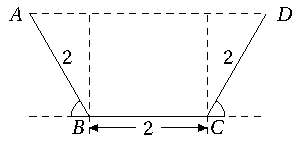
\includegraphics[scale=1]{figure/fig1-3-4.pdf}
				\caption{}\label{fig:1.3.4}
			\end{figure}
			\item 设一抛物线过(\ref{3.142:1})中所求得截面的 $A,D$ 及 $BC$ 中点,记该抛物线与直线段 $AD$ 所围成封闭平面的面积 $\widetilde{S}$,求 $\frac{S}{\widetilde{S}}$;\label{3.142:2}
			\item 若排水沟长为 \SI{1}{m},其横截面原为(\ref{3.142:1})中等腰梯形的形状,因淤泥沉积形成了(\ref{3.142:2})中抛物线的形状. 现清除淤泥,恢复(\ref{3.142:1})中的形状,将淤泥搬运出排水沟,则至少作多少功?(设单位体积的淤泥重为 $\rho$ \si{N/m^3})
		\end{enumerate}
	\end{ti}